\chapter{Generalización y Especialización}

\begin{figure}[h]
  \begin{minipage}{0.5\textwidth}
    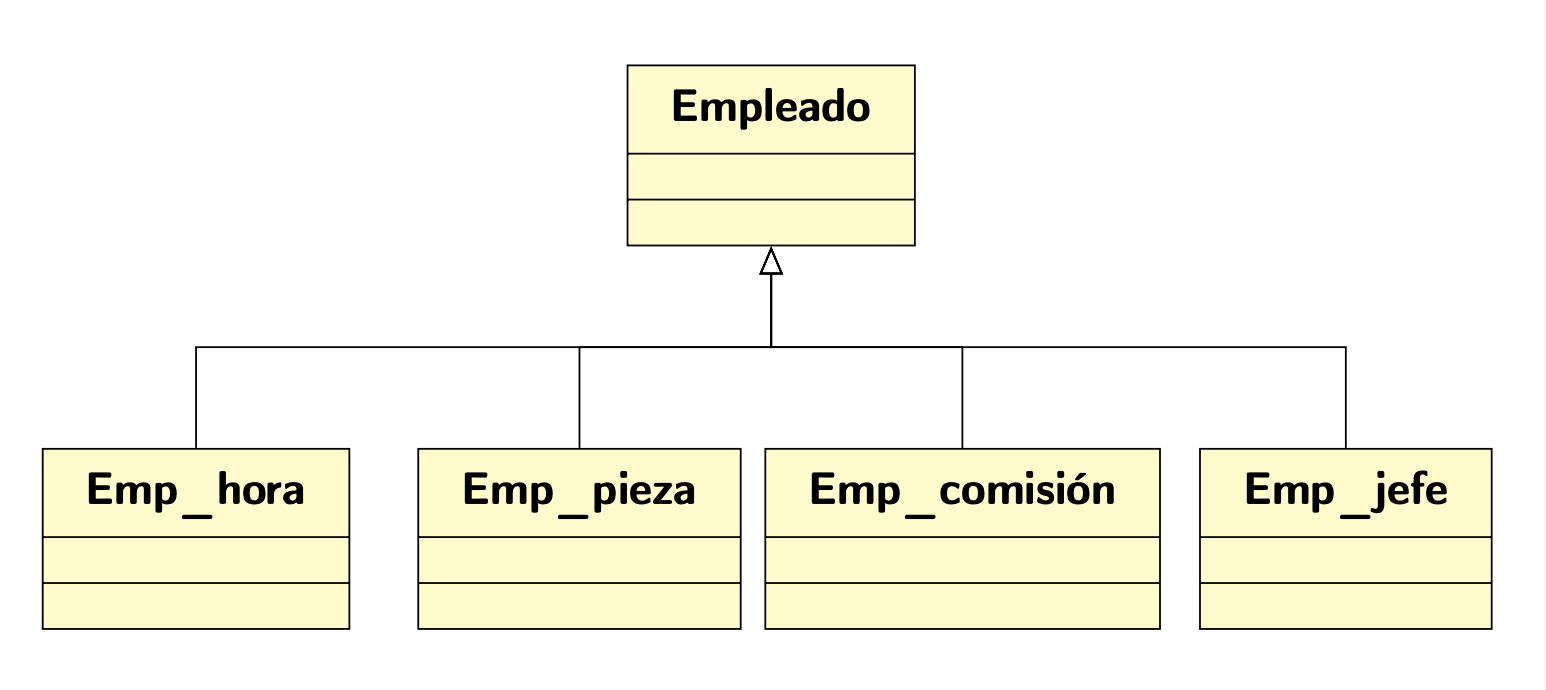
\includegraphics[width=\textwidth]{Imagenes/gen1.png}
    \caption{Diagrama de Clases}
  \end{minipage}
  \begin{minipage}{0.5\textwidth}
      \vspace{-1\baselineskip} % ajusta la posición vertical del texto
Relación ‘ES-UN’ que existe entre una \textit{superclase} y una \textit{subclase}.\\

Una subclase contiene las mismas características que la superclase y atributos extras de la misma.\\

Es lo que en C++ denominamos como herencia, donde la subclase \textit{Emp\_hora}hereda todos los atributos y métodos de la superclase \textit{Empleado} y además estas subclases tendrán métodos propios que no contendrá la superclase.

Las generalizaciones pueden ser \textit{simples} o \textit{múltiples.}
  \end{minipage}
\\

Las subclases se \textbf{generalizan} en una súperclase, al revés la súperclase se \textbf{especializa} en subclases.
\end{figure}
\subsection{En cuanto al diseño}
\subsubsection{Generalización mediante criterios}
\begin{figure}[h]
\centering
  \begin{subfigure}[b]{0.45\textwidth} % 0.4 es el tamaño de la imagen
    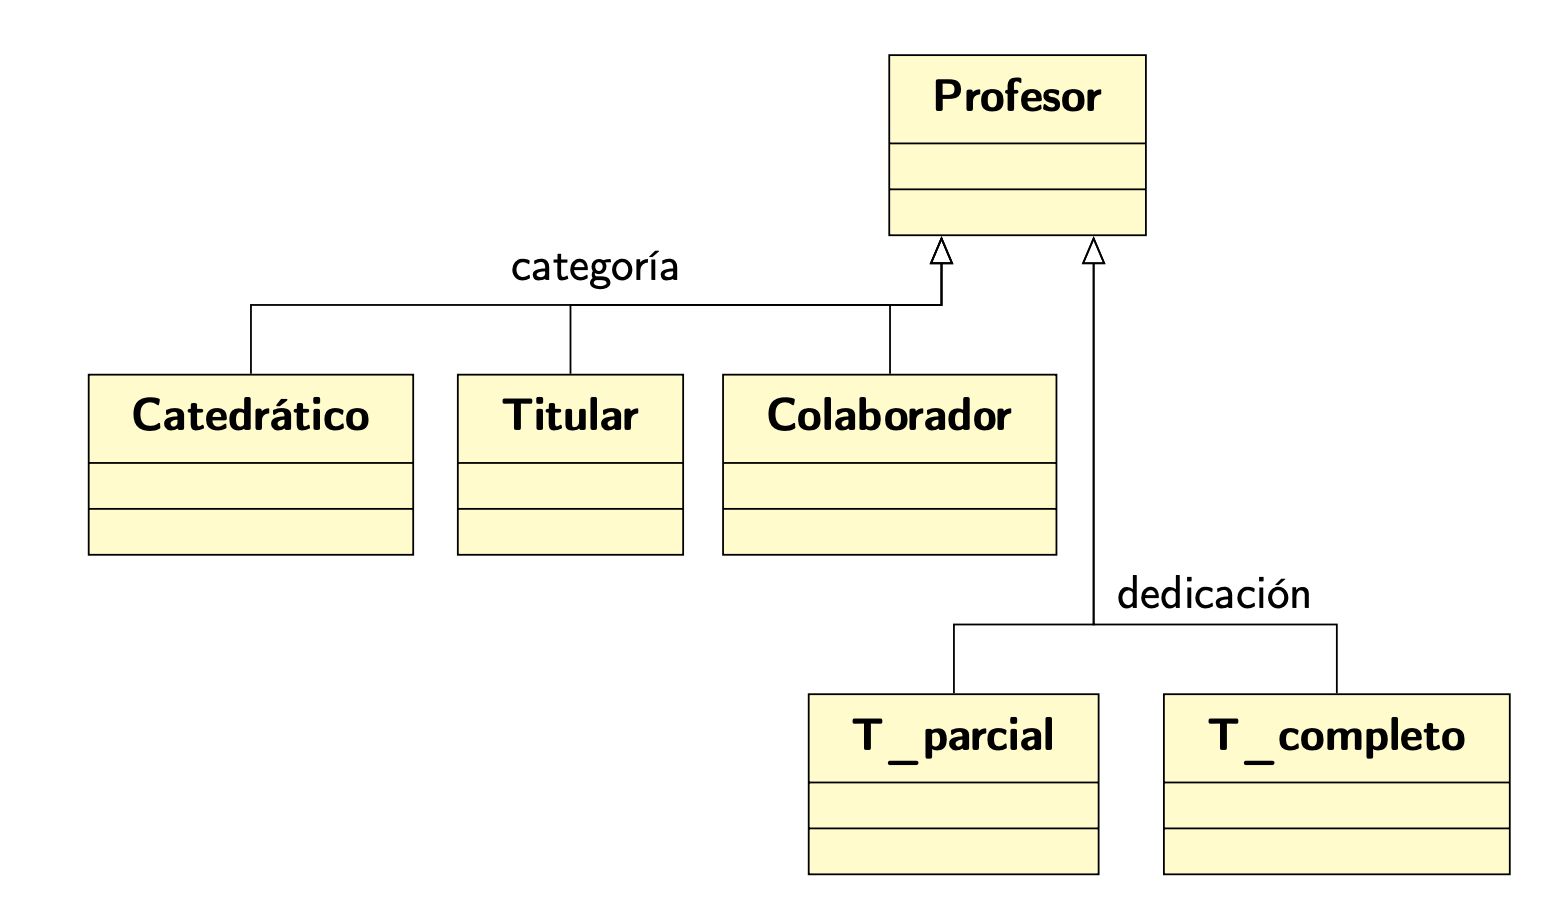
\includegraphics[width=\textwidth]{Imagenes/gen2.png} % 0.9 es el tamaño dentro del espacio anterior
    Podemos generalizar mediante condiciones ‘discriminador’.
    Donde podemos ver que un \textit{profesor} puede tomar diferentes categorías y diferente dedicación.
  \end{subfigure}
  %
  \begin{subfigure}[b]{0.45\textwidth} %Para incluir una segunda figura
  \uline{Ejemplo de Generalización múltiple:}\\
  Vemos que un vehículo puede ser terrestre o acuático y a su vez los terrestres pueden ser un coche o un anfibio, y los acuáticos pueden ser anfibio o barcos.
    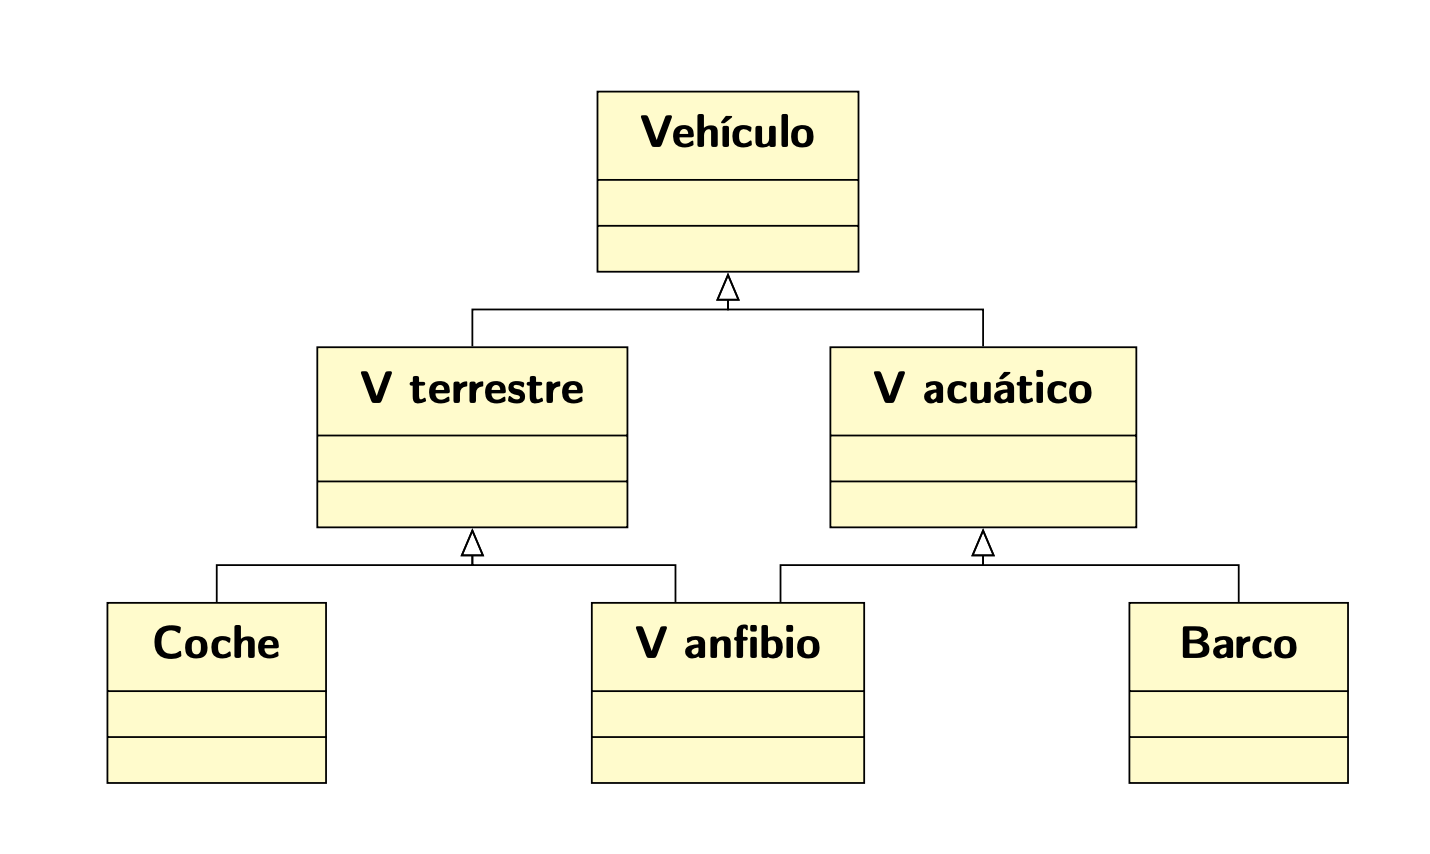
\includegraphics[width=\textwidth]{Imagenes/gen3.png}
  \end{subfigure}
\end{figure}
\end{center}
\newpage
\subsection{En cuando a la implementación}
La programación Orientada a Objetos nos permiten hacer uso de \textbf{herencia} para poder implementar este tipo de relaciones.\\
La herencia es una herramienta muy potente, ya que nos permite la reutilización de código, ya que podemos definir nuevas clases a partir de otras ya definidas.\\
Pero esto puede ser un peligro, ya que podemos confundir una asociación con una \textbf{generalización-especialización}.

Podemos hacernos varias preguntas para saber cual tipo de relación escoger:
\begin{itemize}
	\item ¿Es la clase \textbf{x} un tipo especial de la clase \textbf{y}?
	\item ¿Es posible usar un objeto de la clase \textbf{x} en todas aquellas situaciones en que se emplee un objeto de la clase \textbf{y}?
	\item ¿Y si un objeto de la clase \textbf{x} se va a ejecutar simultáneamente en dos o más relaciones con la clase \textbf{y}, cada una mostrando una vista diferente del mismo?
\end{itemize}

\begin{minipage}[t]{0.5\textwidth}
	\begin{lstlisting}[frame=single]
class clase_derivada[final]:
[accesibilidad] clase_base{
//Declaracion de los miembros de la clase
};
	\end{lstlisting}
Si ponemos final, estamos indicando que esa clase no se va a poder derivar más.
\end{minipage}
\hfill
\begin{minipage}[t]{0.41\textwidth}
Una clase derivada \textbf{NO} hereda:
	\begin{itemize}
		\item Constructores
		\item Destructor
		\item Operadores de asignación
	\end{itemize}
\end{minipage}

La accesibilidad puede ser \texttt{public} , \texttt{private} ó \texttt{protected}.\vspace*{0.4cm}

\begin{minipage}[t]{0.3\textwidth}
	\begin{lstlisting}[frame=single]
class C{
  public:
    int publico;
  protected:
    int protegido:
  private:
    int privado;
};
	\end{lstlisting}
\end{minipage}
\hfill
\begin{minipage}[t]{0.6\textwidth}
	\texttt{Public} → Accesible desde el interior y exterior.\\
	
	\texttt{Protected} → Accesible desde el interior, para funciones amigas de C y desde las clases derivadas de C y sus funciones amigas. Sirven para que los atributos sea accesibles a las clases derivadas pero ocultos al exterior.\\
	
	\texttt{Private}→ Accesible desde el interior y para las funciones amigas de C.
\end{minipage}
\\

Además \texttt{protected} hace que no se cumpla el principio de ocultación de información y las clases estén acopladas, es decir, que debemos comprobar que las clases funcionan para los mismos tipos de datos.\\

\newpage
\begin{center}
	\begin{figure}[h]
	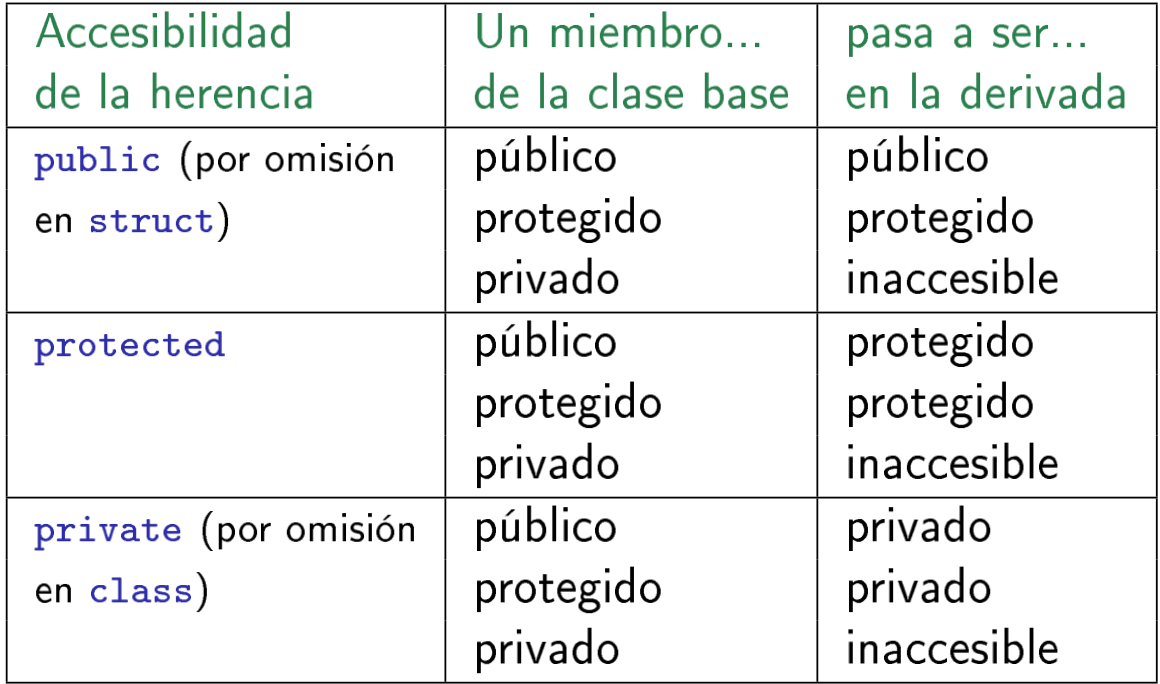
\includegraphics[width=\textwidth]{Imagenes/gen4.png}
	\caption{Modificación de accesibilidad de miembros heredados}
\end{figure}
\end{center}
\vspace*{-1cm}
\end{center}
\left \section{Herencia pública}

Nos sirve para implementar las relaciones de especialización/generalización, es decir, las relaciones ES-UN entre clase base y subclases.
Hereda su comportamiento externo.\\

Esta relación al ser pública, es visible desde el exterior, por tanto, \textit{un objeto de una subclase es también un objeto de la clase base}.
\textit{Podemos realizar conversiones hacia arriba, un objeto de la clase derivada puede convertirse en uno de la clase base, debido a que la clase derivada contiene la misma información que la clase base}.
Pero \textbg{no} se \textit{puede convertir un objeto de la clase base en uno de la derivada debido a que a esta le falta información específica de las clases derivadas}.

\subsubsection{Ejemplo de Herencia Pública:}
Vemos que un \textit{Doctorando} es una especialización de la \textit{clase Estudiante}.\\
Donde la clase \textit{Doctorando} tendría 4 atributos (2 propios y 2 heredados de la clase base) y además un método llamado \texttt{mostrar()}.

Si no ponemos los atributos con los que se crea un objeto de la clase base y este no tiene constructor predeterminado, nos dará un error.
\newpage
\begin{figure}
	\begin{minipage}[t]{0.25\textwidth}
	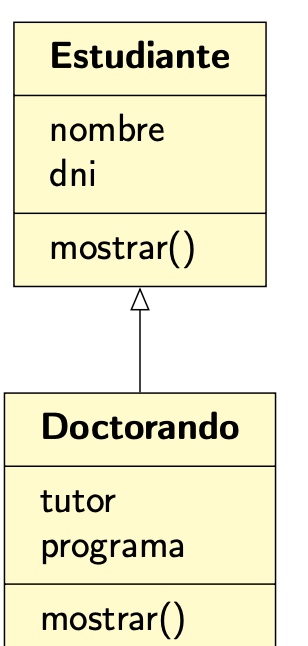
\includegraphics[width=\textwidth]{Imagenes/gen5.png}
	\end{minipage}
\hfill
\begin{minipage}[t]{0.7\textwidth}
\vspace*{-8cm}
	\begin{lstlisting}[frame=single]
class Estudiante{
  public:
    Estudiante(string nombre, int dni);
    void mostrar() const;
  private:
    string nombre; int dni;
    // ...
};

class Doctorando final:public Estudiante
{
  public:
    Doctorando(string nombre,int dni,
	  string tutor, int programa);
    void mostrar() const;
  private:
    string tutor; 
    int programa; 
    // ...
};
	\end{lstlisting}
\end{minipage}
\end{figure}

\begin{center}
	\begin{lstlisting}[frame=single]
Doctorando::Doctorando(string nombre, int dni, string tutor, int programa):Estudiante(nombre, dni), tutor(tutor), programa(programa) {}
  
void Doctorando::mostrar() const{
  // Muestra los datos que posee como estudiante
  Estudiante::mostrar();
  // Y los especícos de su condición de doctorando
  cout << "Programa de doctorado: " << programa << "\n"
       << "Tutor en el programa: " << tutor << endl;
}
\end{lstlisting}
\end{center}

Llamamos al método mostrar que está definido en estudiante, para poder mostrar información sobre el estudiante sea cual sea su especialización.

Si se quiere mostrar la información del \textit{Estudiante} deberíamos de definir observadores debido a que los atributos son \textbf{privados}.

Esto sucede debido a que estamos dentro del ámbito de \textit{Doctorando} y no de \textit{Estudiante}.

Si quitamos el operador de resolución de ámbito, tendríamos una función recursiva.\\
\begin{center}
  \begin{figure}[h]
	\begin{lstlisting}[frame=single]
Estudiante* pe= &e; //puntero a estudiante
pe->mostrar(); //método mostrar de estudiante
pe=&d; //conversión hacia arriba de doctorando a estudiante
pe->mostrar(); //método mostrar de estudiante
/*----------------------------------------------------*/
Doctorando* pd = &d; //puntero a doctorando
pd->mostrar(); //método mostrar de doctorando
pd->Estudiante::mostrar(); //me¡étodo mostrar de estudiante (resolución ámbito)
pd->Doctorando::mostrar(); //método mostrar de doctorando.

/*-----Conversiones entre punteros-----*/
pe = &d; //conversión implicita entre punteros hacia arriba
pd = &e; //Error -> no se puede hacer una conversión implícita hacia abajo
pd= static_cast<Doctorando>(e);//Conversion en T.Compilación corrige lo anterior

/*-----Conversiones entre objetos-----*/
e = d; //Objeto d Doctorando se convierte a un tipo Estudiante
d = e; //Error -> No se puede convertir un objeto e Estudiante (base) a d Doctorando (derivado)
//Tampoco se puede hacer explicita la conversión hacia abajo entre objetos:
	d = Doctorando(e); //Error
	d = static_cast<Doctorando>(e);//Error
	d = reinterpret_cast<Doctorando>(e);//Error
	\end{lstlisting}
	\caption{Ejemplo de herencia pública}\vspace{1cm}
\textit{No se pueden realizar conversiones implícitas hacia abajo entre punteros, estás deben de ser explicitas}.\\

\textit{No se pueden realizar conversiones implícitas ni explícitas hacia abajo entre objetos de las clases base y derivada}.
	\end{figure}
\end{center}

\newpage
\section{Herencia privada}
\vspace{-0.5cm}
Sirven para implementar relaciones “Se implementan con”.\\
Es decir, se hereda la interfaz pública de la base pero en la clase derivada se ocultan debido a que estos pasan a ser \textbf{privados}.\\
Por tanto, la relación entre ambas clases queda oculta para el usuario.

Se puede usar para implementar una \textbf{\textit{relación de composición 1a1}} entre componente y compuesto.

Con la \textit{keyword} \texttt{using} hacemos que el método que especifiquemos pase de ser \textit{privado} a \textit{público} en la clase derivada.

\begin{figure}[h]
	\centering
	\texttt {\textbf{using Clase::nombre\_metodo;}}
	\caption{Declaración de la keyword}
\end{figure}
\section{Jerarquía de Clases}
La \textbf{herencia simple} nos permite definir jerarquía entre las clases relacionadas, donde una clase se deriva solamente de una clase base, y la cadena de derivación no es circular.


\begin{figure}[h]
	\begin{minipage}[t]{0.4\textwidth}
		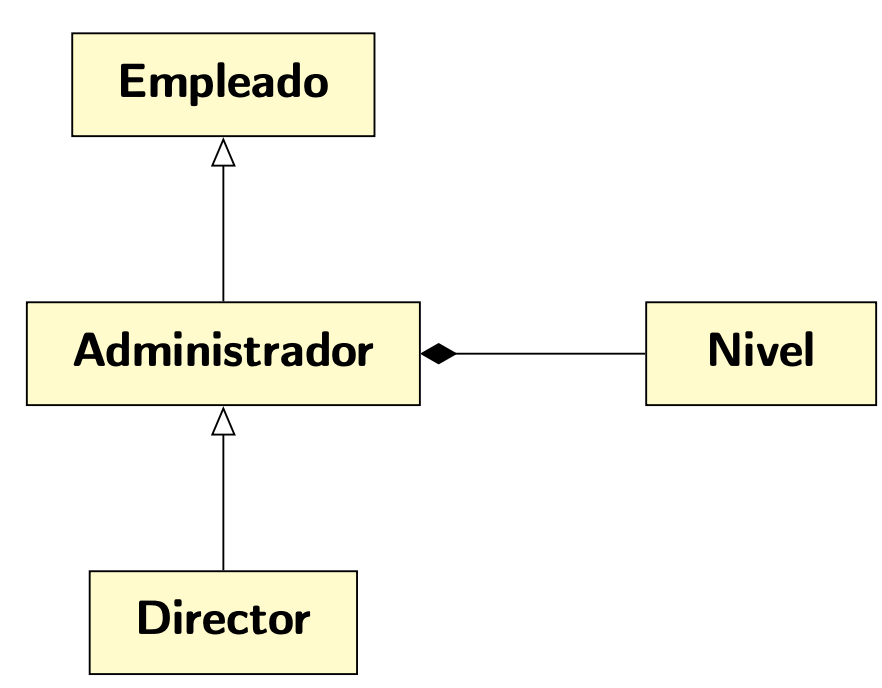
\includegraphics[width=\textwidth]{Imagenes/gen6.png}
		\caption{Ejemplo de herencia simple}
	\end{minipage}
	\hfill
	\begin{minipage}[t]{0.55\textwidth}
\vspace{-4.6cm}
		\begin{lstlisting}[frame=single]
class Empleado{//..};
class Administrador: public Empleado {
protected:
	Nivel nivel;
	// ...
};
class Director final: public Administrador { // ...};
		\end{lstlisting}
	\end{minipage}
\end{figure}

\section{Herencia múltiple}
\vspace{-0.55cm}
\begin{center}
	\begin{figure}[h]
	\centering
	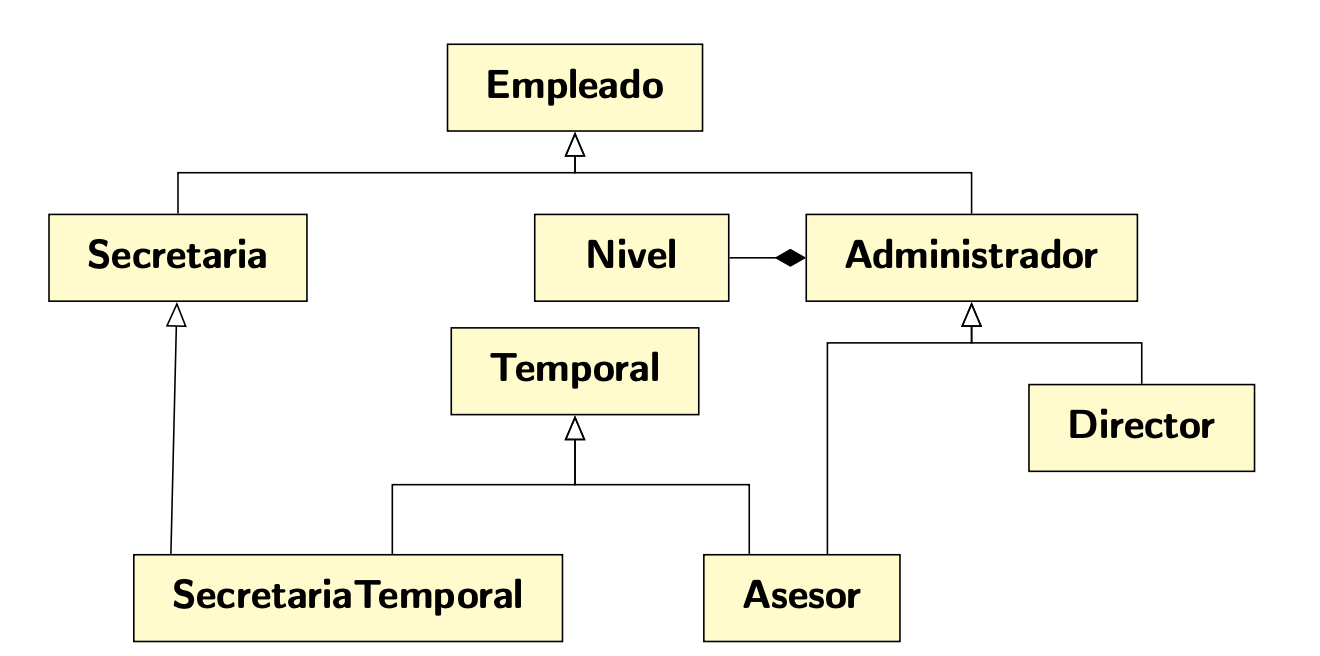
\includegraphics[width=\textwidth]{Imagenes/gen7.png}
\end{figure}
\end{center}
Una clase base puede tener varias clases derivadas, además la cadena de derivación puede ser circular. Podemos crear una nueva clase combinando características de varias clases.

Vemos que la clase \textit{Secretaria Temporal} se deriva de \textit{Temporal} y \textit{Secretaría}, por ejemplo.
Se declara ampliando la lista de derivación.
\newpage
\subsection{Código del ejemplo anterior}
\begin{center}
	\begin{lstlisting}[frame=single]
class Temporal {//...};
class Secretaria: public Empleado {//...};
class SecretariaTemporal final: public Temporal, public Secretaria {//...};
class Asesor final: public Temporal, public Administrador {//...};
\end{lstlisting}
\end{center}

\begin{minipage}[t]{0.45\textwidth}
\subsubsection{Orden de inicialización de los objetos en herencia múltiple}
1. Constructores de las clases bases en el orden de la lista de derivación.\\

2. Constructores de los atributos en el orden declarado dentro de la clase.\\

3. Se ejecuta el constructor de la clase derivada.

\end{minipage}
\hfill
\begin{minipage}[t]{0.45\textwidth}
\subsubsection{Orden de destrucción de los objetos en herencia múltiple}
1. Se llama al destructor de la clase derivada.\\

2. Se llama al destructor de las clases base en orden inverso al que han sido declarados.
\end{minipage}
\newpage
\section{Ambigüedades al heredar miembros sobrecargados\\ en Herencia múltiple}
Si los métodos no están en el mismo ámbito, no hay sobrecargar por tanto el compilador no sabría que método sobrecargado usar.

Cuando tenemos métodos que tienen el mismo nombre pero definidos en ámbitos diferentes, a la hora de llamarlos tenemos ambigüedades, por eso llamamos al operador de resolución de ámbito → hacemos que no haya sobrecarga.

Para que haya sobrecarga, nos llevamos todos esos métodos con el mismo nombre al mismo ámbito mediante la keyword \texttt{using}.
\begin{center}
\begin{figure}[h]
	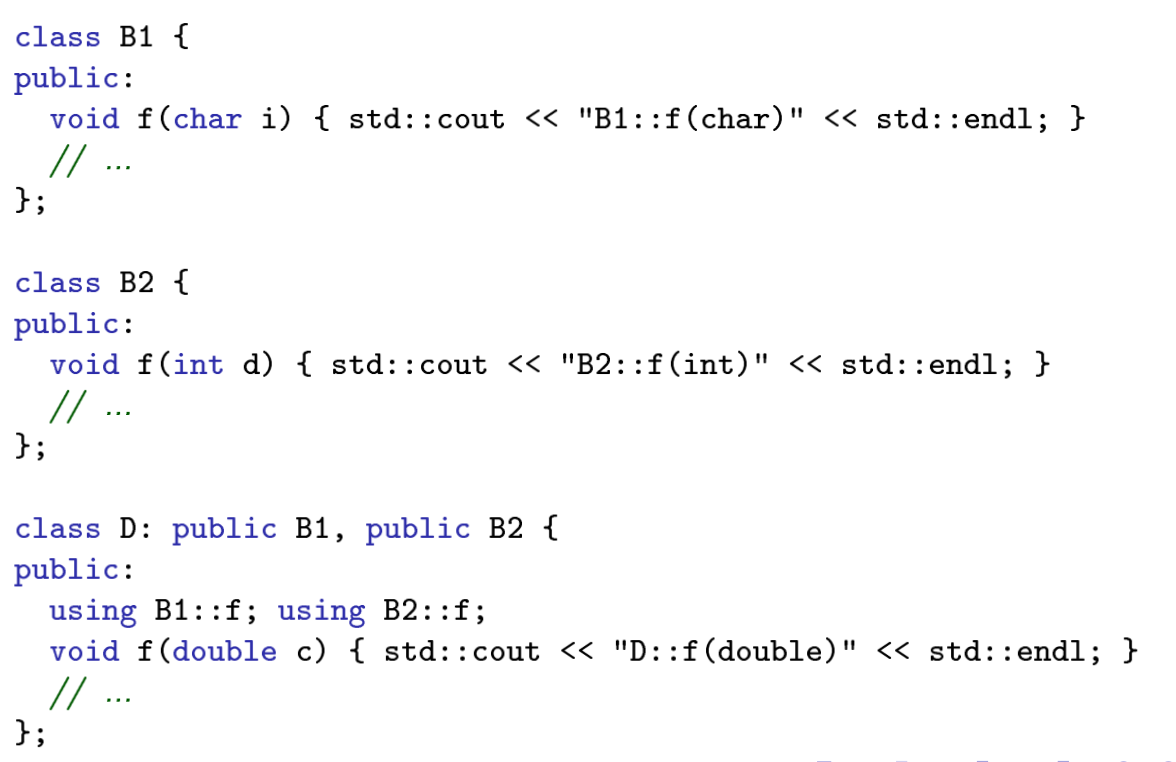
\includegraphics[width=\textwidth]{Imagenes/gen8.png}
\end{figure}
\end{center}

\newpage

\section{Herencia virtual}
\begin{center}
	\begin{figure}[h]
	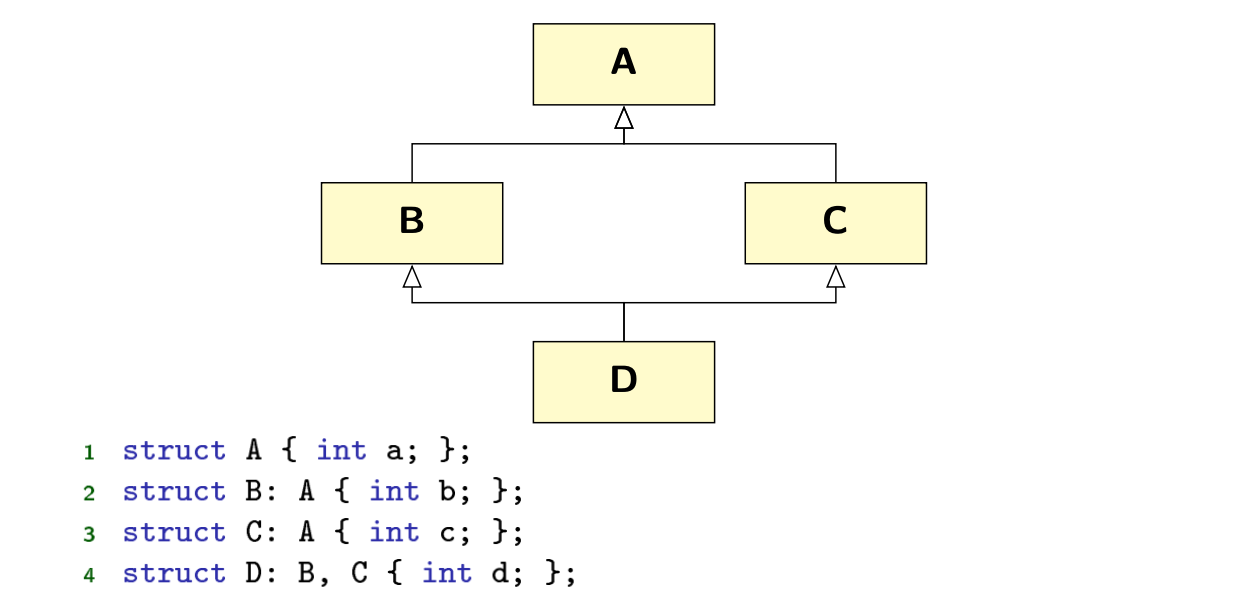
\includegraphics[width=\textwidth]{Imagenes/gen9.png}
	\caption{Problema del diamante}
\end{figure}
\end{center}
Para resolver el problema del diamante, podemos hacer uso de la herencia virtual, donde D tiene 2 miembros de la clase A, donde si no lo definimos así encontraríamos una ambigüedad → \texttt{d.B::a} y \texttt{d.C::a}.  
\begin{center}
	\begin{figure}[h]
	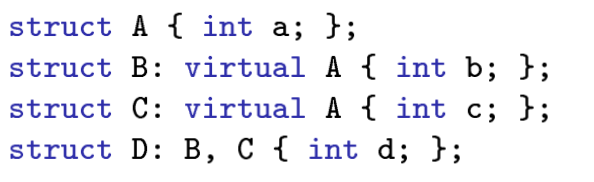
\includegraphics[width=\textwidth]{Imagenes/gen10.png}
	\caption{Ejemplo de herencia virtual}
\end{figure}
\end{center}
Mediante la \textit{keyword} \texttt{virtual} delante de la herencia hacemos que no haya duplicidad y D solamente tendrá un miembro \texttt{a}.

\newpage
\section{Realización}
Es la relación entre una \textit{interfaz} y una clase.

Una interfaz es una clase que \textbf{solo} declara métodos no atributos, ni constructores ni destructores.

Se realiza mediante herencia, donde esa clase interfaz es una clase abstracta y es superclase.

Por ejemplo, podemos tener una interfaz \texttt{pila} y luego especializaciones de maneras de implementarla dicha pila.

Para ello, la clase que queremos que sea una interfaz / clase abstracta debe de tener como mínimo un método definido como \textbf{virtual puro}, es decir:
\begin{center}
	\texttt{virtual tipo\_metodo nombre\_metodo(parámetros)=0}. 

\end{center} 
Encapsula todos los métodos que serán comunes a las clases especializadas de la misma.